\section{Dimensionierung}
Folgend wird beschrieben, wie die Komponenten ausleget und welche Überlegungen bei der Auslegung gemacht wurden.\\
Die Dimensionierung wurde mit einer Exceltabelle durchgeführt, welche im elektronischen Anhang \ref{e:Dimensionierung} einsehbar ist.

\subsection{Boden - Mittleres Raumelement}
\label{Boden}
Der Fussboden des Solar Butterflys soll als Sandwichstruktur realisiert werden, wobei als Deckschicht Aluminiumblech und als Kern geschäumtes Ocean-PET verwendet werden soll. Der Fussboden muss die Personenlasten aufnehmen und auf das Chassis übertragen. Weiter sieht das zum Zeitpunkt der Durchführung dieser Arbeit verfolgte Konzept vor, dass die seitlichen Raumelemente während der Fahrt über den Boden mit dem Rest der Struktur verbunden und befestigt werden. Im Rande des Bodens sollen abschnittweise Aluminiumprofile oder Purenit-Hartschaum eingebettet werden, an welchen die seitlichen Raumelemente befestigt werden können.\\
Zu Beginn der Ausarbeitung des Konzeptes wurden umrahmende Aluminiumprofile aus dem Fahrzeugbau zur Konstruktion in Betracht gezogen, welche auf Platten mit einer Dicke von 25 mm passen. Eine erste Annahme der Dicke des Bodens wurde so getroffen, dass diese in die besagten Profile passen. Über eine Absprache mit einem Experten aus dem Wohnmobilbau wurde in Erfahrung gebracht, dass in Wohnmobilen häufig Fussböden mit einer Dicke von 30 mm, mit einer Dicke der Deckschichten von 1 mm, verbaut werden. [QUELLE] Weiter wurde mitgeteilt, dass die erste Abschätzung der Dicke von 25 mm eine plausible sei und weiterverfolgt werden soll.

Um die getroffene Annahme zu überprüfen und die Dicke der Deckschichten zu bestimmen, wurden für zwei Belastungsfälle Berechnungen angestellt. Die unterschiedlichen Belastungsfälle sowie deren Idealisierungen der Lagerung und Krafteinleitung sind in der Abbildung \ref{Boden Idealisierung} dargestellt. Die Beiden Lager A und B stellen dabei die beiden Längsträger des Chassis dar.

\begin{figure}[!ht]
  \centering
    \begin{subfigure}{.5\textwidth}
      \centering
      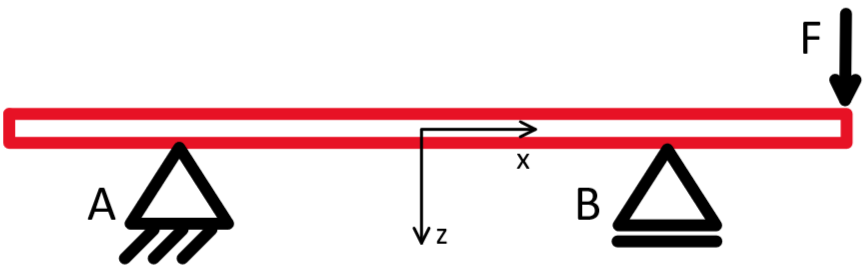
\includegraphics[width=.8\linewidth]{04_figures/Boden Fall1.png}
      \caption{Belastungsfall 1}
      \label{Belastungsfall 1}
    \end{subfigure}%
    \begin{subfigure}{.5\textwidth}
      \centering
      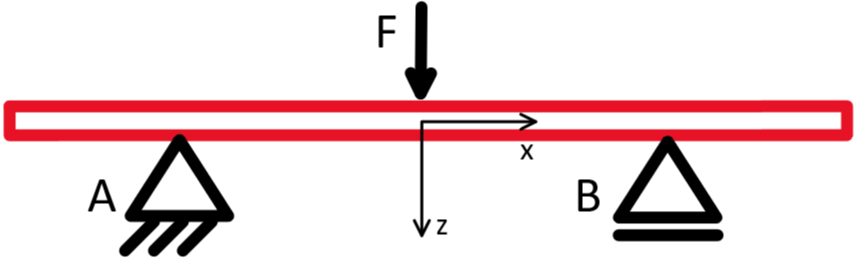
\includegraphics[width=.8\linewidth]{04_figures/Boden Fall2.png}
      \caption{Belastungsfall 2}
      \label{Belastungsfall 2}
    \end{subfigure}%
  \caption{Darstellung der beiden Belastungsfällen und deren Idealisierungen}
\label{Boden Idealisierung}
\end{figure}

Als Belastung wird eine Masse von 200 kg gewählt, welche auf einen 1000 mm langen Bodenabschnitt eingeleitet wird. Der Boden hat eine Breite von 2050 mm und der Abstand zwischen den Lagern beträgt 1410 mm. Als Kernmaterial wird das leichteste dem Projekt zur Verfügung stehende Schaummaterial \emph{Airex T92.60} verwendet. Das technische Datenblatt des Materials ist im elektronischen Anhang \ref{e:Airex} zu finden. In der Abbildung \ref{Boden QM} sind die Querkraft- und Biegemomentenverläufe der beiden Belastungsfälle dargestellt.

\begin{figure}[H]
  \centering
    \begin{subfigure}{.5\textwidth}
      \centering
      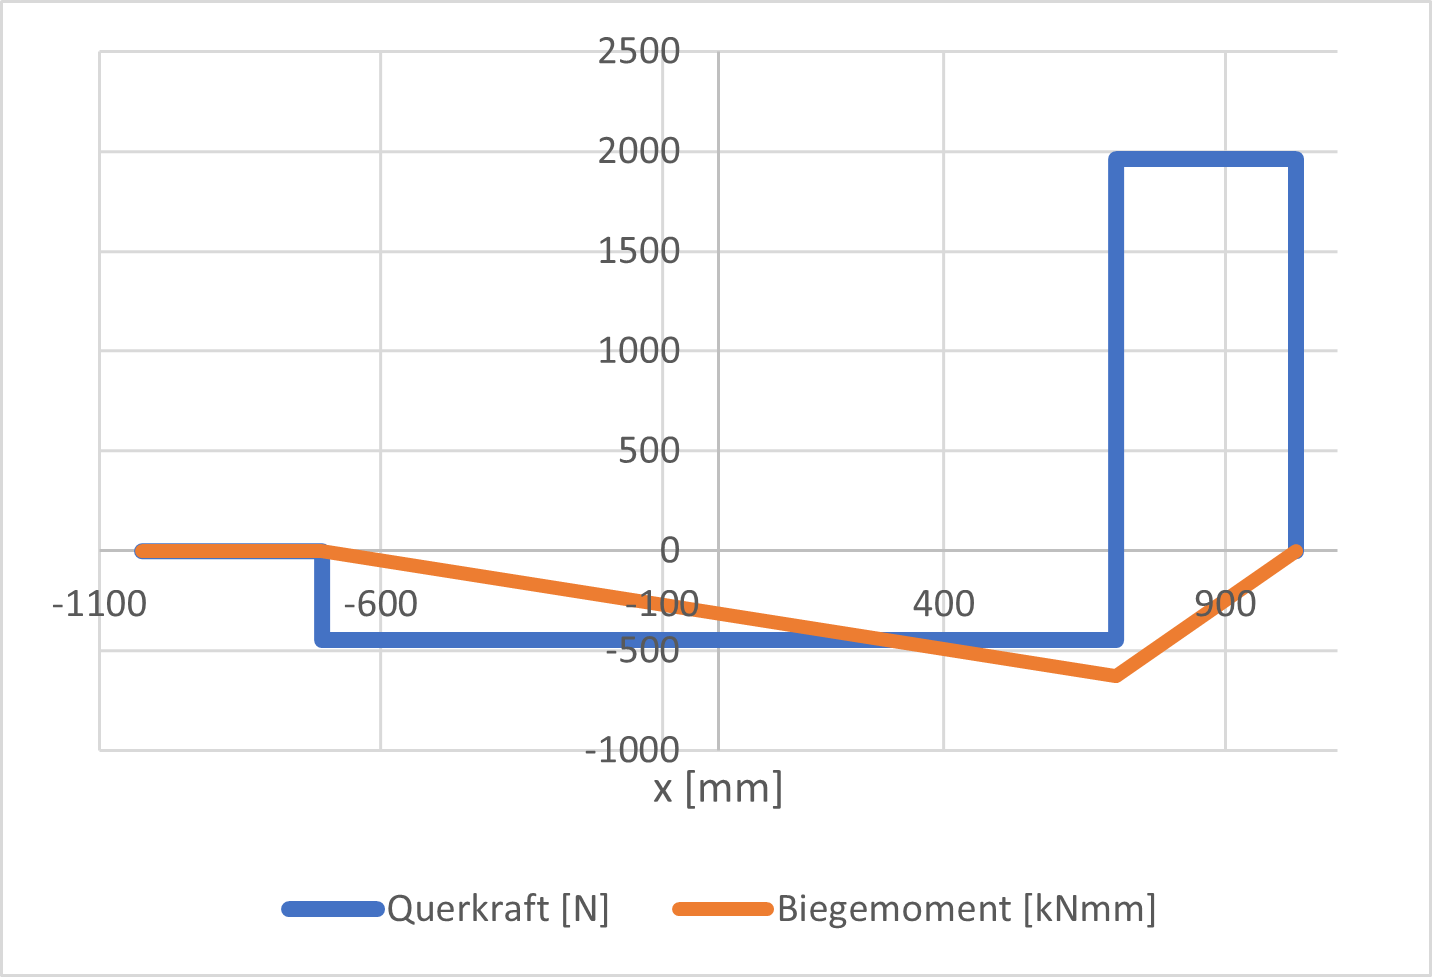
\includegraphics[width=.98\linewidth]{04_figures/Boden QM1.png}
      \caption{Belastungsfall 1}
      \label{Boden QM1}
    \end{subfigure}%
    \begin{subfigure}{.5\textwidth}
      \centering
      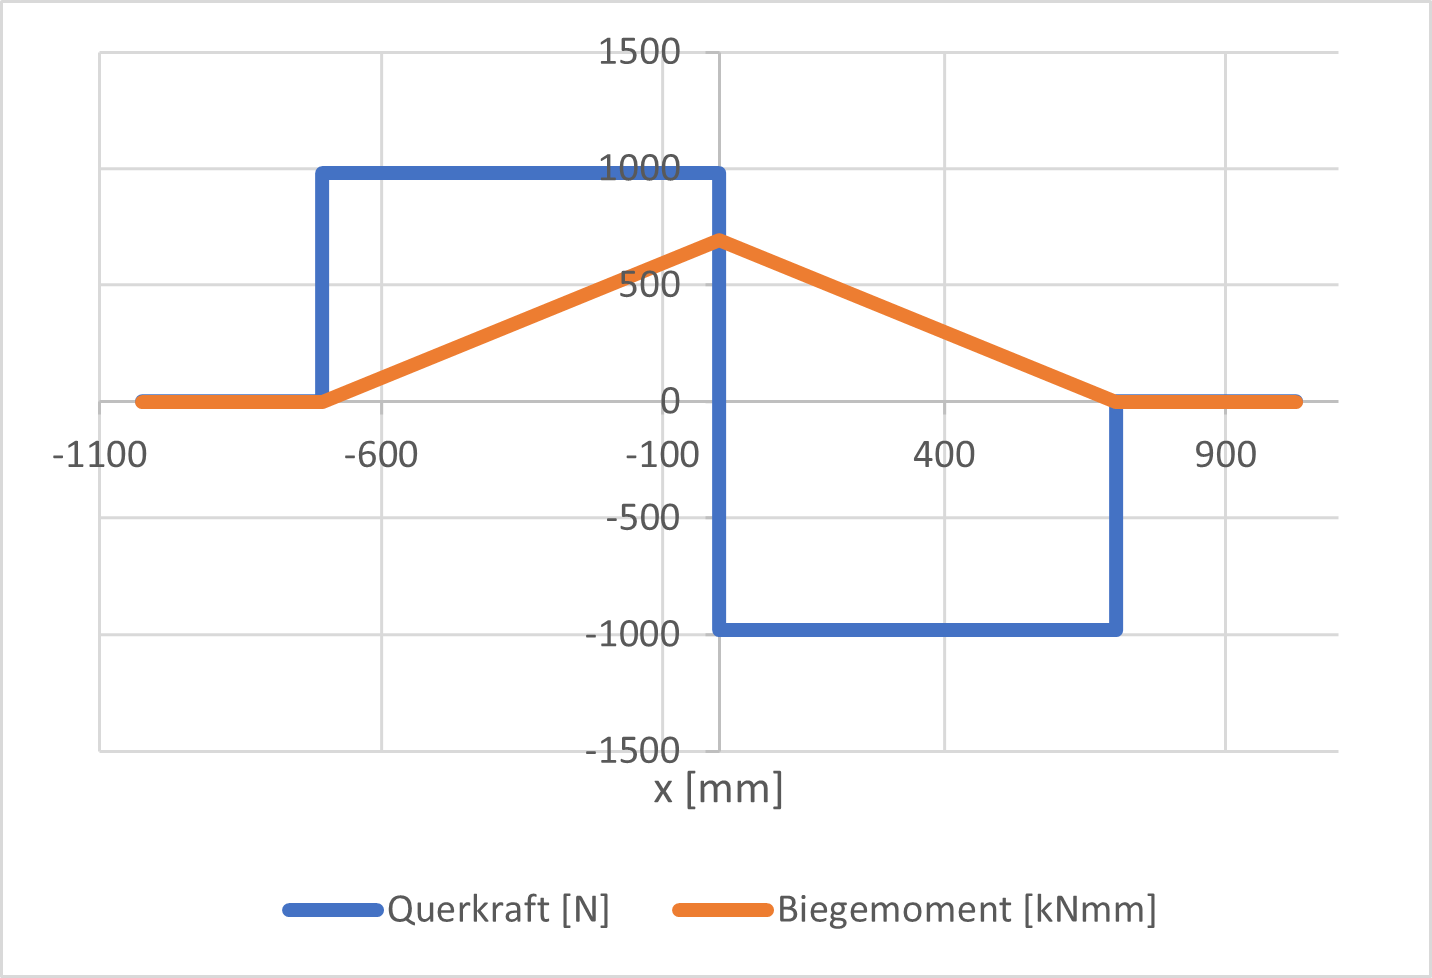
\includegraphics[width=.98\linewidth]{04_figures/Boden QM2.png}
      \caption{Belastungsfall 2}
      \label{Boden QM2}
    \end{subfigure}%
  \caption{Querkraft- und Biegemomentenverläufe der Bodenplatten}
\label{Boden QM}
\end{figure}

Mit einer Deckschicht von 0.36 mm Dicke wird im Belastungsfall 2, gemäss der Formel \ref{Spannung in Deckschicht}, eine Spannung von 80 MPa erreicht, was dem Design-Allowable von Aluminium entspricht. Die Druckspannungen, welche an den Auflageflächen der Bodenplatte auf den Chassis herrschen, liegen tiefer als 0.1 MPa und stellen keine kritischen Spannungen für das Kernmaterial dar. Weiter stellen das Schubbeulen der Kernschicht sowie das Knittern der Deckschicht keine Gefahren dar. Sie treten bei Spannungen von 248, respektive 168 MPa auf (aus den Formeln \ref{Schubbeulen} und \ref{Knittern}).\\

Als Missbrauchslastfall wird das Betreten des Bodens einer Person welche ``spitze Schuhe'' trägt betrachtet. Steht eine 75 kg schwere Person auf einer Querschnittsfläche von 1000 $mm^2$ (Kreisfläche mit einem Durchmesser von rund 35 mm), wird die minimal erreichbare Druckfestigkeit des Kernmaterials von 0.75 MPa überschritten. Durch die mittragenden Deckschichten ist die effektiv belastete Querschnittsfläche des Kernmaterials jedoch grösser und die Belastung entsprechend kleiner. Dennoch ist es wahrscheinlich, dass im Verlaufe der Lebensdauer des Solar Butterflys ungünstigere Umstände eintreffen und dadurch höhere Belastungen erreicht werden, wodurch der Boden Schaden nehmen könnte. Die Verwendung des nächstfesteren Kernmaterials (Minimale Druckfestigkeit von 1.1 MPa) würde das Risiko eines Schadens reduzieren, hätte jedoch eine Erhöhung des Gewichtes von rund 20 kg zur Folge. (Berechnet mit 40 $m^2$ Bodenfläche.)\\
Von der Firma \emph{3A-Composites} wird empfohlen, Aluminium-Deckschichten mit einer Dicke von 1 mm zu verwenden, da Sie selbst Deckschichten in dieser Ausführung verwenden und gute Erfahrungen gemacht wurden. Weiter wurden Bedenken bezüglich der Verwendung dünneren Deckschichten geäussert.\\
Da das Überschreiten des Gewichtslimits des Solar Butterflys ein Projektrisiko darstellt, wird, um das Gewicht zu reduzieren, von der Empfehlung abgewichen und dünnere Deckschichten verwendet. Auf der Unterseite des Bodens wird eine Dicke von 0.6 mm und auf der begehbaren Oberseite eine Dicke von 0.8 mm gewählt. Mit dieser Wahl der Dicken der Deckschichten kann das Gewicht des Bodens, im Vergleich zu beidseitig 1 mm dicken Deckschichten, um rund 65 kg reduziert werden.

Ein weiterer Aspekt des Bodens, welcher berücksichtigt wird, ist dessen Nachgiebigkeit unter Belastung. Der Boden soll sich beim Begehen nicht zu stark verformen\footnote{Für die Verformbarkeit des Bodens wurde keine klare Anforderung definiert. Die zulässige Verformbarkeit wird nach eigenem Ermessen abgeschätzt.}.  Mit den gewählten Dicken der Deckschichten und der zuvor erwähnten Belastung von 200 kg, würde eine Kernschicht mit einer Dicke von rund 11.5 mm genügen, um die Design-Allowables der Deckschichten nicht zu überschreiten. Der Boden würde sich bei dieser Wahl jedoch um 22 mm Durchbiegen. Bei einer Dicke des Bodens von 25 mm (Dicke des Kernes von 23.6 mm) verformt sich der Boden maximal lediglich um rund 6 mm (Belastungsfall 2), was als zulässig beurteilt wird.

Bei der Wahl des leichten Kernmaterials und den dünnen Deckschichten wird, da viel Gewicht gespart werden kann, bewusst ein Risiko eingegangen. Es ist wahrscheinlich, dass der Boden im Verlauf der Lebensdauer des Solar Butterflys Schaden, in Form von eingedrückten Stellen, nehmen wird. Die Auswirkungen eines solchen Schadens sind jedoch gering. So stellen allfällige Schäden, auf Grund der überdimensionierten Deckschichten (überdimensionierten im Vergleich zu 0.36 mm), keine Gefahr für die Integrität der Gesamtstruktur dar. Weiter können die eingedrückten Stellen mit geringem Aufwand mit einer Spachtelmasse oder Füller ausgebessert werden, sodass der Solar Butterfly weiterhin optisch ansprechend bleibt.

\subsection{Dach - mittleres Raumelement}
\label{sec:Dach}
Das Dach des mittleren Raumelementes besteht aus zwei Aluminium-Rechteckprofilen und vier Solarpanelen, welche auf die Längsträger geklebt werden. Die Solarpanelen ihrerseits sind 14.5 mm dicke Sandwichkonstruktionen bestehend aus PET-Schaum und Deckschichten aus glasfaserverstärktem Kunststoff (GFK). Das Dach hat eine Breite von 2.1 Meter und eine Länge von rund 5.3 Meter. In der Abbildung \ref{img:Dach} ist das mittlere Raumelement des Solar Butterflys dargestellt.\\

\begin{figure}[h]
  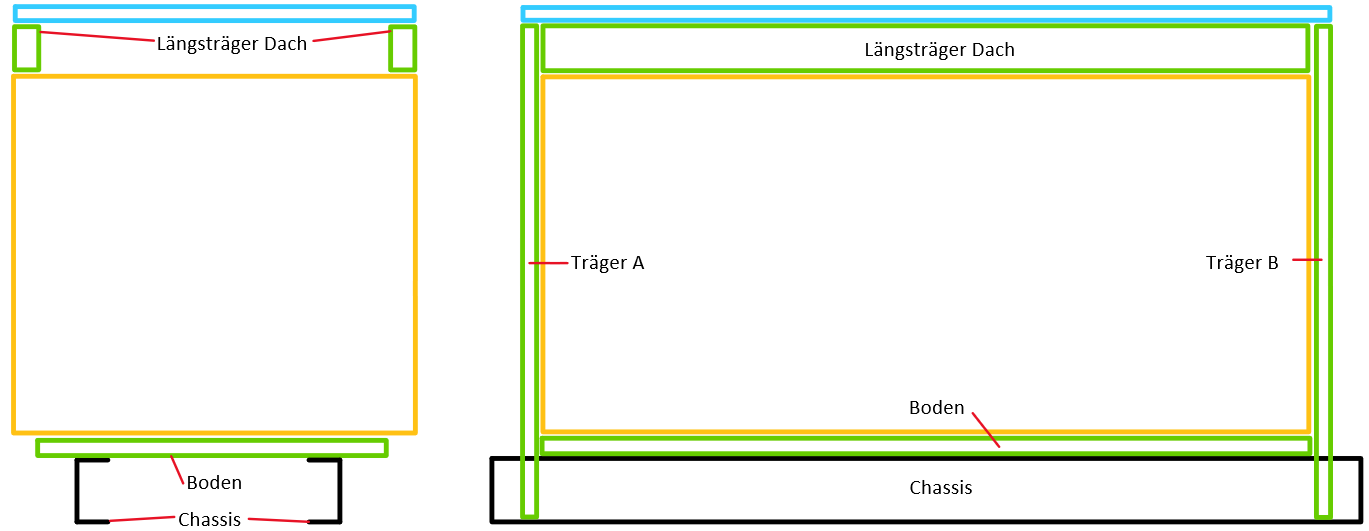
\includegraphics[width=\linewidth]{04_Figures/Dach.png}
  \caption{Darstellung des mittleren Raumelementes}
  \label{img:Dach}
\end{figure}

Die Längsträger des Daches werden so ausgelegt, dass die Verformung des Daches durch dessen Eigengewicht die Funktion der seitlichen Raumelemente nicht einschränkt. Es wird von einer maximal zulässigen Verformung von 50 mm ausgegangen. Um die Verformung des Daches zu berechnen, wird die Biegesteifigkeit des Daches gemäss der Formel \ref{eq:1}, unter Berücksichtigung der unterschiedlichen Steifigkeiten der Materialien, berechnet. Dabei wird 50\% der breite der Solarpanelen als mittragend berücksichtigt. Als Belastung wird das Eigengewicht als Flächenlast eingeführt. Bei der Wahl des Profils gilt es, dessen Höhe minimal zu halten, da die Höhe der Längsträger direkt die Höhe der ausziehbaren Raumelementen reduzieren.\\
Bei der Wahl eines Profils mit 40 mm Höhe, 25 mm Breite und einer Wandstärke von 2 mm, hängt das Dach bei einer gelenkigen Lagerung (vgl. Abbildung \ref{Dach Idealisierung}) um 40 mm durch. Um die Spannungen in den Längsträgern und der oberen Deckschicht der Panelen zu berechnen, wurden die Lagerkräfte sowie der Querkraft und Biegemomentenverlauf berechnet, welcher in der Abbildung \ref{Dach QM} abgebildet ist. Gemäss der Formel \ref{eq:2} ergeben sich in den Längsträgern maximale Zugspannungen von 19 MPa und in den Deckschichten der Panelen Druckspannungen von 2.2 MPa.\\
Bei einer zusätzlichen Belastung von rund 370 kg, gleichmässig verteilt auf die Fläche des Daches, wird in den Längsträgern die zulässige statische Spannung von 160 MPa erreicht. Die Spannungen in der oberen Deckschicht der Solarpanele ergibt sich zu 19 MPa. Die zusätzliche Belastung könnte z.B. aufgrund von Schneefall auftreten.

\begin{figure}[h]
\centering
\begin{minipage}{.4\textwidth}
  \centering
  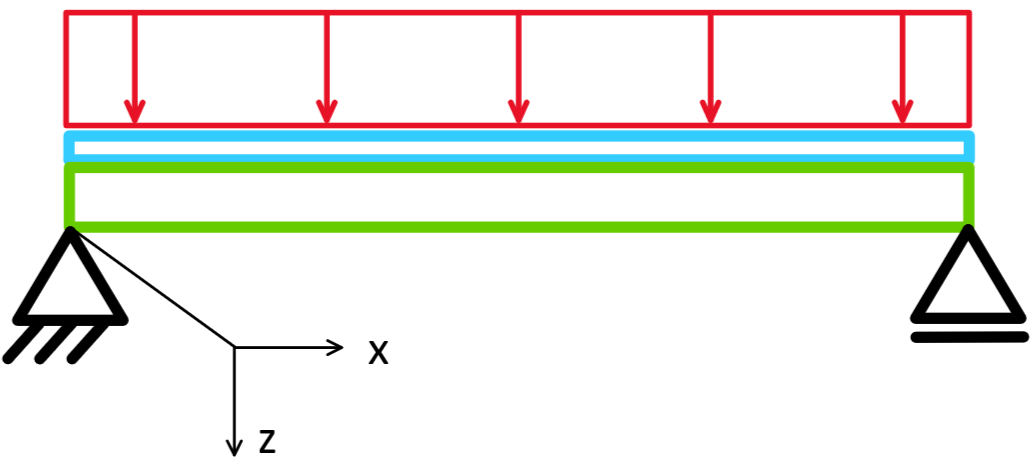
\includegraphics[width=.98\linewidth]{04_figures/Dach Idealisierung.png}
  \caption{Lagerung des Daches und idealisierte Krafteinleitung}
  \label{Dach Idealisierung}
\end{minipage}%
\begin{minipage}{.6\textwidth}
  \centering
  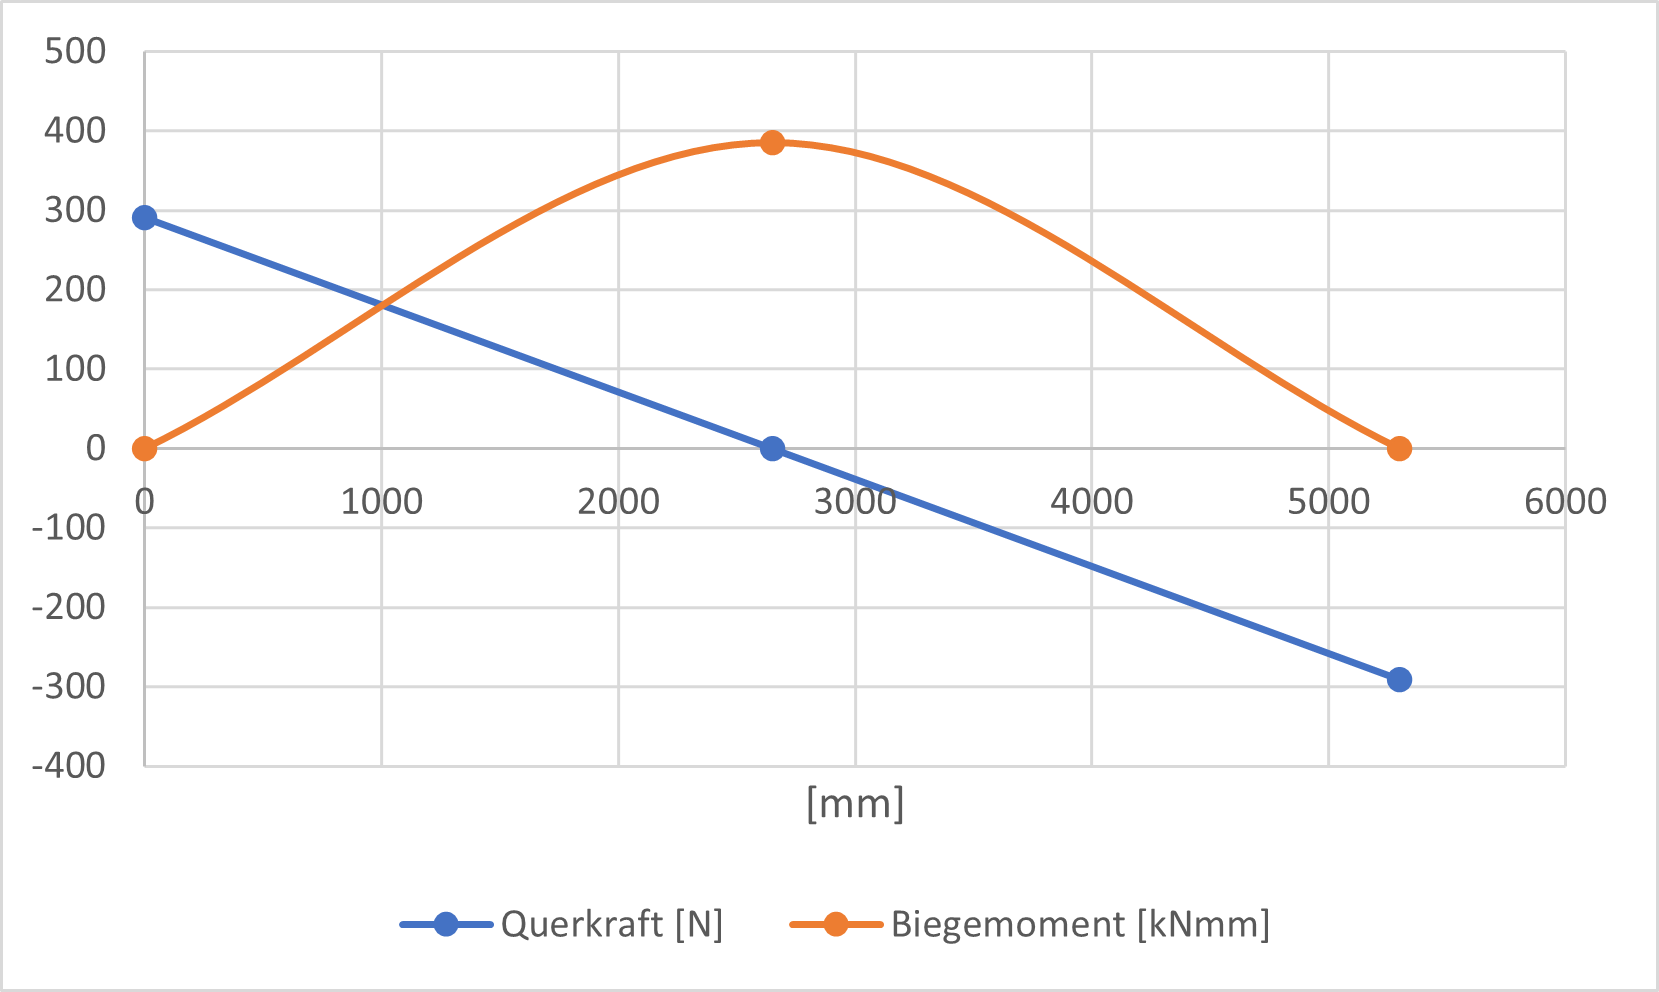
\includegraphics[width=.98\linewidth]{04_figures/Dach QM.png}
  \caption{Querkraft- und Biegemomentenverlauf}
  \label{Dach QM}
\end{minipage}
\end{figure}


\subsection{Solarpanelen - Reihe D}
Die Äusserste Reihe der Solarpanelen werden über Teleskopscharniere befestigt und mittels Pneumatikzylinder ausgeschoben. Um \emph{Bacher} bei der Auswahl der Teleskopscharniere zu unterstützen wurden Handrechnungen und einige einfachere FEM-Analysen mit jeweils unterschiedlichen Lagerungen durchgeführt. Ausgelesen wurden die totalen Verformungen sowie die unterschiedlichen Lagerreaktionen. Die entsprechenden FEM-Dateien sind im elektronischen Anhang \ref{e:Panelen} angefügt.

\begin{figure}[h]
  \centering
  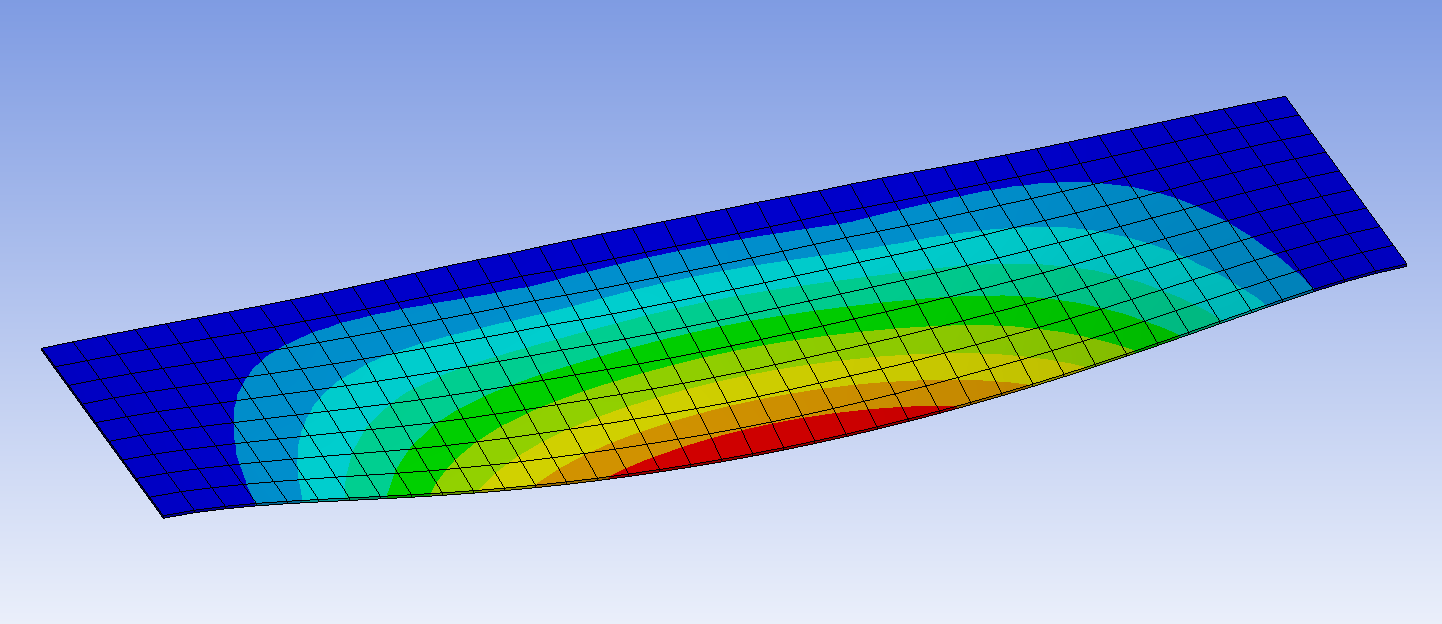
\includegraphics[width=.6\linewidth]{04_figures/Panelen Verformung.png}
  \caption{Beispiel-Bild einer FEM-Analyse der Solarpanele Reihe D}
  \label{Panelen Verformung}
\end{figure}
\newpage
